\documentclass[a4paper,11pt]{article}
\usepackage[latin1]{inputenc}
\usepackage{ulem}
\usepackage{a4wide}
\usepackage[dvipsnames,svgnames]{xcolor}
\usepackage[pdftex]{graphicx}
\usepackage{hyperref}
\usepackage{array}

\newcommand{\MYp}[1]{ {\color[rgb]{0.392,0.392,0.392}#1} }
\newcommand{\MYunder}[1]{ {\color[rgb]{0.2,0.209,0.3}\underline{#1}} }

\begin{document}


\includegraphics{fdi.jpg}
\newline
\newline
\newline
\MYp{\Huge Aut\'{o}mata de entrada}
\begin{center}
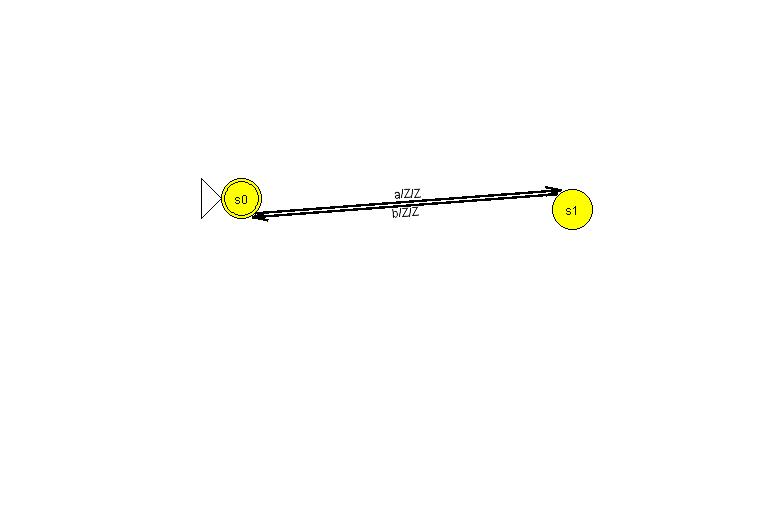
\includegraphics[width=\textwidth]{imagenEntrada.jpg}
\end{center}
\MYp{\Huge Gram\'{a}tica de entrada simplificada\newline
\newline
}
\begin{center}\begin{tabular}{ m{15cm} }

\noindent {\bf Variables: }[S, A, B, C, D, E, F, G, H, I, J] \\
{\bf Variable Inicial: }S \\ 
{\bf S\'{i}mbolos Terminales: }[a, b] \\ 
{\bf Producciones: }{D=[F,D, a,H, a,J, /], E=[a,H], F=[a,I], G=[a,J, /], A=[F,A], B=[F,B], S=[A, B, C, D], C=[F,C], H=[b,E], I=[b,F], J=[b,G]} \\ 
\end{tabular}
\end{center}
\newpage\MYp{\Huge Gr\'amatica}
\newline

\begin{center}\begin{tabular}{ m{15cm} }

\noindent {\bf Variables: }[S, A, B, C, D, E, F, G, H, I, J] \\
{\bf Variable Inicial: }S \\ 
{\bf S\'{i}mbolos Terminales: }[a, b] \\ 
{\bf Producciones: }{D=[F,D, a,H, a,J, /], E=[a,H], F=[a,I], G=[a,J, /], A=[F,A], B=[F,B], S=[A, B, C, D], C=[F,C], H=[b,E], I=[b,F], J=[b,G]} \\ 
\end{tabular}
\end{center}

\begin{center}
\begin{tabular}{||c||c||c||c||c||c||c||c||c||c||c||}
\hline
\hline
- & A & B & C & D & E & F & G & H & I & J \\
\hline
\hline
S & - & X & X & X & X & - & - & - & - & - \\
\hline
\hline
A & - & - & - & - & - & - & X & - & - & - \\
\hline
\hline
B & - & - & - & - & - & - & X & - & - & - \\
\hline
\hline
C & - & - & - & - & - & - & X & - & - & - \\
\hline
\hline
D & - & - & - & - & - & - & X & - & - & - \\
\hline
\hline
E & - & - & - & - & - & - & - & - & - & - \\
\hline
\hline
F & - & - & - & - & - & - & - & - & - & - \\
\hline
\hline
G & - & - & - & - & - & - & - & - & - & - \\
\hline
\hline
H & - & - & - & - & - & - & - & - & - & - \\
\hline
\hline
I & - & - & - & - & - & - & - & - & - & - \\
\hline
\hline
J & - & - & - & - & - & - & - & - & - & - \\
\hline
\hline
\end{tabular}
\end{center}

\MYp{\Huge Gr\'amatica}
\newline

\begin{center}\begin{tabular}{ m{15cm} }

\noindent {\bf Variables: }[S, A, B, C, D, E, F, G, H, I, J] \\
{\bf Variable Inicial: }S \\ 
{\bf S\'{i}mbolos Terminales: }[a, b] \\ 
{\bf Producciones: }{D=[F,D, a,H, a,J, /], E=[a,H], F=[a,I], G=[a,J, /], A=[F,A], B=[F,B], S=[F,A, B, C, D], C=[F,C], H=[b,E], I=[b,F], J=[b,G]} \\ 
\end{tabular}
\end{center}

\begin{center}
\begin{tabular}{||c||c||c||c||c||c||c||c||c||c||c||}
\hline
\hline
- & A & B & C & D & E & F & G & H & I & J \\
\hline
\hline
S & - & - & X & X & X & - & X & - & - & - \\
\hline
\hline
A & - & - & - & - & - & - & X & - & - & - \\
\hline
\hline
B & - & - & - & - & - & - & X & - & - & - \\
\hline
\hline
C & - & - & - & - & - & - & X & - & - & - \\
\hline
\hline
D & - & - & - & - & - & - & X & - & - & - \\
\hline
\hline
E & - & - & - & - & - & - & - & - & - & - \\
\hline
\hline
F & - & - & - & - & - & - & - & - & - & - \\
\hline
\hline
G & - & - & - & - & - & - & - & - & - & - \\
\hline
\hline
H & - & - & - & - & - & - & - & - & - & - \\
\hline
\hline
I & - & - & - & - & - & - & - & - & - & - \\
\hline
\hline
J & - & - & - & - & - & - & - & - & - & - \\
\hline
\hline
\end{tabular}
\end{center}

\MYp{\Huge Gr\'amatica}
\newline

\begin{center}\begin{tabular}{ m{15cm} }

\noindent {\bf Variables: }[S, A, B, C, D, E, F, G, H, I, J] \\
{\bf Variable Inicial: }S \\ 
{\bf S\'{i}mbolos Terminales: }[a, b] \\ 
{\bf Producciones: }{D=[F,D, a,H, a,J, /], E=[a,H], F=[a,I], G=[a,J, /], A=[F,A], B=[F,B], S=[F,A, F,B, C, D], C=[F,C], H=[b,E], I=[b,F], J=[b,G]} \\ 
\end{tabular}
\end{center}

\begin{center}
\begin{tabular}{||c||c||c||c||c||c||c||c||c||c||c||}
\hline
\hline
- & A & B & C & D & E & F & G & H & I & J \\
\hline
\hline
S & - & - & - & X & X & - & X & - & - & - \\
\hline
\hline
A & - & - & - & - & - & - & X & - & - & - \\
\hline
\hline
B & - & - & - & - & - & - & X & - & - & - \\
\hline
\hline
C & - & - & - & - & - & - & X & - & - & - \\
\hline
\hline
D & - & - & - & - & - & - & X & - & - & - \\
\hline
\hline
E & - & - & - & - & - & - & - & - & - & - \\
\hline
\hline
F & - & - & - & - & - & - & - & - & - & - \\
\hline
\hline
G & - & - & - & - & - & - & - & - & - & - \\
\hline
\hline
H & - & - & - & - & - & - & - & - & - & - \\
\hline
\hline
I & - & - & - & - & - & - & - & - & - & - \\
\hline
\hline
J & - & - & - & - & - & - & - & - & - & - \\
\hline
\hline
\end{tabular}
\end{center}

\MYp{\Huge Gr\'amatica}
\newline

\begin{center}\begin{tabular}{ m{15cm} }

\noindent {\bf Variables: }[S, A, B, C, D, E, F, G, H, I, J] \\
{\bf Variable Inicial: }S \\ 
{\bf S\'{i}mbolos Terminales: }[a, b] \\ 
{\bf Producciones: }{D=[F,D, a,H, a,J, /], E=[a,H], F=[a,I], G=[a,J, /], A=[F,A], B=[F,B], S=[F,A, F,B, F,C, D], C=[F,C], H=[b,E], I=[b,F], J=[b,G]} \\ 
\end{tabular}
\end{center}

\begin{center}
\begin{tabular}{||c||c||c||c||c||c||c||c||c||c||c||}
\hline
\hline
- & A & B & C & D & E & F & G & H & I & J \\
\hline
\hline
S & - & - & - & - & X & - & X & - & - & - \\
\hline
\hline
A & - & - & - & - & - & - & X & - & - & - \\
\hline
\hline
B & - & - & - & - & - & - & X & - & - & - \\
\hline
\hline
C & - & - & - & - & - & - & X & - & - & - \\
\hline
\hline
D & - & - & - & - & - & - & X & - & - & - \\
\hline
\hline
E & - & - & - & - & - & - & - & - & - & - \\
\hline
\hline
F & - & - & - & - & - & - & - & - & - & - \\
\hline
\hline
G & - & - & - & - & - & - & - & - & - & - \\
\hline
\hline
H & - & - & - & - & - & - & - & - & - & - \\
\hline
\hline
I & - & - & - & - & - & - & - & - & - & - \\
\hline
\hline
J & - & - & - & - & - & - & - & - & - & - \\
\hline
\hline
\end{tabular}
\end{center}

\MYp{\Huge Gr\'amatica}
\newline

\begin{center}\begin{tabular}{ m{15cm} }

\noindent {\bf Variables: }[S, A, B, C, D, E, F, G, H, I, J] \\
{\bf Variable Inicial: }S \\ 
{\bf S\'{i}mbolos Terminales: }[a, b] \\ 
{\bf Producciones: }{D=[F,D, a,H, a,J, /], E=[a,H], F=[a,I], G=[a,J, /], A=[F,A], B=[F,B], S=[F,A, F,B, F,C, F,D, a,H, a,J, /], C=[F,C], H=[b,E], I=[b,F], J=[b,G]} \\ 
\end{tabular}
\end{center}

\begin{center}
\begin{tabular}{||c||c||c||c||c||c||c||c||c||c||c||}
\hline
\hline
- & A & B & C & D & E & F & G & H & I & J \\
\hline
\hline
S & - & - & - & - & - & - & X & - & - & - \\
\hline
\hline
A & - & - & - & - & - & - & X & - & - & - \\
\hline
\hline
B & - & - & - & - & - & - & X & - & - & - \\
\hline
\hline
C & - & - & - & - & - & - & X & - & - & - \\
\hline
\hline
D & - & - & - & - & - & - & X & - & - & - \\
\hline
\hline
E & - & - & - & - & - & - & - & - & - & - \\
\hline
\hline
F & - & - & - & - & - & - & - & - & - & - \\
\hline
\hline
G & - & - & - & - & - & - & - & - & - & - \\
\hline
\hline
H & - & - & - & - & - & - & - & - & - & - \\
\hline
\hline
I & - & - & - & - & - & - & - & - & - & - \\
\hline
\hline
J & - & - & - & - & - & - & - & - & - & - \\
\hline
\hline
\end{tabular}
\end{center}

\MYp{\Huge Gr\'amatica}
\newline

\begin{center}\begin{tabular}{ m{15cm} }

\noindent {\bf Variables: }[S, A, B, C, D, E, F, G, H, I, J] \\
{\bf Variable Inicial: }S \\ 
{\bf S\'{i}mbolos Terminales: }[a, b] \\ 
{\bf Producciones: }{D=[a,I,D, a,H, a,J, /], E=[a,H], F=[a,I], G=[a,J, /], A=[a,I,A], B=[a,I,B], S=[a,I,A, a,I,B, a,I,C, a,I,D, a,H, a,J, /], C=[a,I,C], H=[b,E], I=[b,F], J=[b,G]} \\ 
\end{tabular}
\end{center}

\begin{center}
\begin{tabular}{||c||c||c||c||c||c||c||c||c||c||c||}
\hline
\hline
- & A & B & C & D & E & F & G & H & I & J \\
\hline
\hline
S & - & - & - & - & - & - & - & - & - & - \\
\hline
\hline
A & - & - & - & - & - & - & - & - & - & - \\
\hline
\hline
B & - & - & - & - & - & - & - & - & - & - \\
\hline
\hline
C & - & - & - & - & - & - & - & - & - & - \\
\hline
\hline
D & - & - & - & - & - & - & - & - & - & - \\
\hline
\hline
E & - & - & - & - & - & - & - & - & - & - \\
\hline
\hline
F & - & - & - & - & - & - & - & - & - & - \\
\hline
\hline
G & - & - & - & - & - & - & - & - & - & - \\
\hline
\hline
H & - & - & - & - & - & - & - & - & - & - \\
\hline
\hline
I & - & - & - & - & - & - & - & - & - & - \\
\hline
\hline
J & - & - & - & - & - & - & - & - & - & - \\
\hline
\hline
\end{tabular}
\end{center}

\MYp{\Huge Gram\'{a}tica final simplificada}
\newline\begin{center}\begin{tabular}{ m{15cm} }

\noindent {\bf Variables: }[S, A, B, C, D, E, F, G, H, I, J] \\
{\bf Variable Inicial: }S \\ 
{\bf S\'{i}mbolos Terminales: }[a, b] \\ 
{\bf Producciones: }{D=[a,I,D, a,H, a,J, a,I], E=[a,H], F=[a,I], G=[a,J], A=[a,I,A], B=[a,I,B], S=[a,I,A, a,I,B, a,I,C, a,I,D, a,H, a,J, /, a,I], C=[a,I,C], H=[b,E], I=[b,F], J=[b,G, b]} \\ 
\end{tabular}
\end{center}

\end{document}